\documentclass[fsharpNotes.tex]{subfiles}
\graphicspath{ {./figures/} }

\begin{document}
\chapter{Data Structures}
\label{chap:lists}

\abstract{
  Data structures is an organisation of collections of data, such that operations on them are efficient. In earlier chapters, we have already looked at some examples, e.g.,
  \begin{itemize}
  \item strings which are variable length sequences of characters and which was discussed in \Cref{chap:calculator},
  \item tuples which are fixed length sequences of values of variable types and which was  discussed in \Cref{sec:tuples},
  \item lists which are a variable length sequences of values of identical type and which was  discussed in \Cref{chap:lists}, and
  \item stacks which are specialized lists, where values can only be added and removed from its head, and which was discussed in \Cref{sec:stack}.
  \end{itemize}
In this chapter, we will further consider the following data structures:
  \begin{itemize}
  \item \idx{queues} which are a specialized lists, where elements can added to the end of the list and removed from its head,
  \item \idx{trees} which are hierarchical orderings of data of variable number of values of identcial types,
  \item \idx{graphs} which are networks of nodes,
  \item \idx{sets} which are an unordered collection of unique values of the identical type, and
  \item \idx{hash maps} which are mappings between sets of keys into sets of values. 
  \end{itemize}
  These data structures have a long history and are often discussed from an abstract point of view in terms of their conceptual interface and from a computational complexity point of view, where details of their implementation is stressed. The above mentioned data structures occur frequently alone or in combination in many programming solutions and form a solid basis for solving problems by programming. Some of these data structures have their predefined modules in F\# but not all. In this chapter we will give a brief introduction to each.}


\section{Queues}
A queue consists of a sequence values which can be added to its end and removed from its front as illustrated in \Cref{fig:queue}.
\begin{figure}
  \centering
  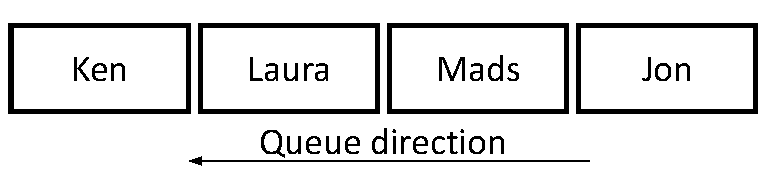
\includegraphics[width=0.6\linewidth]{queue}
  \caption{A queue is a sequence of elements, where new elements are added to the end and removed fromt the front.}
  \label{fig:queue}
\end{figure}
Queues appear often in real life: Standing in line at a shop counter, orders await in a queue for their turn to be shipped in an online shop, students waiting to be examined at oral examinations. The operation of a purely functional queues is given in \Cref{queueInterface}.
%
\fsSignature{queue}{queueInterface}{Basic operations on a queue.}{}
%
These queues are called \emph{(purely) functional} because the enqueue and dequeue operations return a \emph{new} queue they are called, without destroying the old queue. Mutable queues are more common, where en- and dequeueing updates the value of a queue as a side-effect. See \Cref{sec:mutableValues} for more on mutable values.

As of the writing of this book, the standard collection of Fsharp libraries does not include a queues module, but they can easily be implemented using lists. For example, a queue of integers is implemented in \Cref{queueImplementation}.
%
\fsImplementation{queue}{queueImplementation}{Implementing a functional queue using lists.}{}
%
A simple application using this queue is shown in \Cref{queueApp}
%
\fs{queueApp}{An application of the Queue module.}
%
Note that this implementation, the computational complexity of all but \lstinline{enqueue} is $\mathcal{O}(1)$, while \lstinline{enqueue} is $\mathcal{O}(n)$, where $n$ is the length of the list, since it relies on list concatenation. Faster implementations exists but are beyond the scope of this book.

\section{Trees}
\begin{figure}
  \centering
  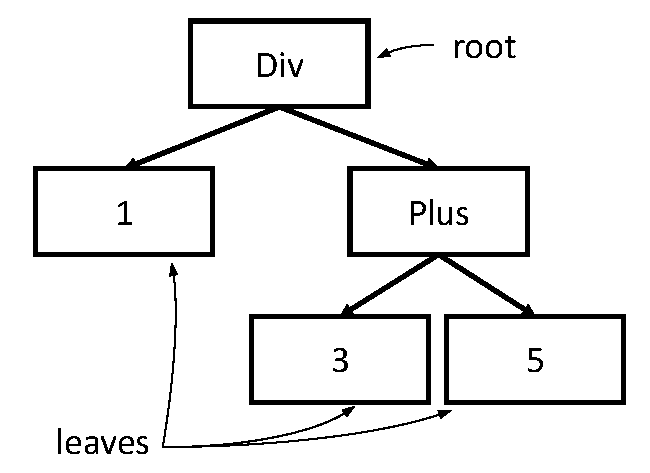
\includegraphics[width=0.45\linewidth]{tree}
  \caption{A tree consists of a hiearchically organized nodes. The top is called the root and the bottom nodes are leaves.}
  \label{fig:queue}
\end{figure}

\section{Graphs}

\section{Sets}

\section{Hash Maps}

\section{Key concepts and terms in this chapter}
Summary text about the key concepts from this chapter
\begin{itemize}
\item \ldots
\end{itemize}
\end{document}
